\setchapterpreamble[u]{\dictum[Monkey in Kubo and the Two Strings]{If you have no memory, how can you be certain of anything?}\bigskip}
\chapter{Introduction}

Memory in its different forms is an important aspect of human, but also animal cognition.
For example, it allows animals to return to previously visited water and food locations \parencite{vorhees2014}, allows to act more optimally in situations similar to prior experiences, or to avoid dangerous situations.
In this sense, memory allows for adaptation on a faster time scale than genetic selection.
This is especially important in unstable and changing environments.
In humans, memory is also important to form social relationships, a shared culture, and even a functioning society.
For example, strategies in the repeated prisoner's dilemma depend on working memory capacity \parencite{milinski1998}.
Moreover, memory contributes to our individual sense of self \parencite{prebble2013}.
Apart from this functional perspective, an addressable memory is also important from a computational perspective.
It allows for a more compact implementation of many computational processes than a pure state machine could achieve \parencite{gallistel2009}.
Overall, the storage of information over time is a fundamental requirement in many cognitive systems.

Accordingly, there is a long history of memory research.
The well-known primacy and recency effect (discussed in more detail in \cref{sec:exp-findings}) have already been described by \textcite{Robinson1926}.
Nevertheless, there are still many open questions.
One important challenge that memory systems have to solve is the so-called \emph{stability-plasticity dilemma} \parencite{Abraham2005}.
On the one hand, there is a need to quickly form new memories, sometimes even with a single exposure known as \emph{one-shot learning}.
On the other hand, such high plasticity can easily lead to overwriting of old memories rendering memory systems useless.
\Textcite{Buzsaki1989} and others proposed multi-stage memory models to address this where different memory systems are in place for different timescales with different levels of plasticity.

Despite this, much of experimental research and modeling treat different memory systems as isolated.
This simplifies the analysis on a certain level, but to get a general understanding of memory as a whole the results need to be integrated at some point.
Furthermore, many models of memory or learning focus on either small scale neural changes without any direct connection to behaviour or on the other extreme of describing behaviour with mathematical equations, but no solid grounding in biological plausibility.
So it is not only important to integrate our understanding of memory systems, but also to bridge the gap from neural mechanisms to behaviour.
With this thesis I advance the understanding in this direction by proposing a model integrating short- and long-term memory and thus modeling their interaction.
Moreover, I implement the model as a spiking neural network to ensure biological plausibility, while at the same time matching behavioural data.

While this is still limited with regard to the variety of memory systems covered, there are promising long-term prospects from a better understanding of human memory.
Many forms of memory loss are currently untreatable.
However, diseases associated with aging, like Alzheimer's, significantly impair the function of memory and are getting more common as our life-span increases due to other medical and nutritional advances.
A better understanding of memory might allow us to devise better treatments or even stop and reverse the memory detoriation.
A potential route to this are memory implants that have already been demonstrated in rats by \textcite{Berger2011}.
For these sort of implants, an understanding of how memories are encoded is at least helpful if not crucial.

These are certainly strong motivators for research into memory, but it is also worthwhile to advance our general understanding of how the human brain works.
An important step in testing our current understanding of the brain was the Spaun model \parencite{Eliasmith2012}.
A spiking neural network of 2.5 million neurons, thus grounded in biology, that can perform 8 different tasks.
Like a real brain it gets sensory input (low resolution black and white symbols) and produces a behavioural motor output with a simulated arm.
The number of tasks it can perform demonstrates that it is not a specialized model for a single task, but can switch between different tasks like a real brain.
Obviously, Spaun is still much simpler (and has much less neurons) than an actual brain and still far from a full understanding of the brain.
But it incorporates a number of qualitative key aspects such as the ability to switch task, making human-like errors, and being implemented in a spiking neural network.
However, one key aspect is still missing.
While it can perform working memory dependent tasks and has simple reinforcement learning, it is missing a declarative and episodic long-term memory.
The work in this thesis can also be seen as a step toward implementing a model of such memory for the future integration in even larger scale models combining further key aspects of cognition.


\section{Behavioural characterization of memory}
Memory systems have been characterized in different and sometimes contradictory ways.
However, one commonly used distinction is made along two orthogonal dimensions:
by timescale and by type of information stored.
On the timescale axis one can differentiate between \emph{short-term memory (STM)} lasting for up to tens of seconds and \emph{long-term memory (LTM)} which can last between hours to decades \parencite{chaudhuri2016}.
However, there is no single agreed upon definition of the exact boundaries.
Sometimes the term \emph{very long-term memory (vLTM)} is used in addition to STM and LTM for memory that exceeds LTM \parencite{solso1998}.

Another use of these terms defines STM as memory being maintained through sustained neural firing, while LTM is realized by synaptic-weight changes.
The volatility of sustained neural firing explains why in this use of terms, STM usually corresponds to information maintained on shorter timescales than in LTM\@.
In this classification, vLTM would correspond to information that has been consolidated from hippocampus to neo-cortical connections.
Moreover, the term working memory (WM) is often used to refer to active representations that allow direct mental manipulation.
In this thesis, I will use the latter definition of these terms.

When classifying memory by type of information, a representation as a tree structure can be helpful (\cref{fig:memtypes}).
On the highest level, we have the distinction between implicit and explicit memory.
Implicit memory does not allow for conscious access.
A typical example is procedural or motor memory like the exact muscle contractions for keeping balance when riding a bike.
Explicit memory allows for conscious access and is further subdivided into declarative and episodic memory.
The declarative memory allows us to store and reproduce facts like the birthday of a friend, whereas the episodic memory provides a recollection of life experiences.
Here, I will focus on declarative memory as this type of memory has been well studied in many memory experiments.
\begin{figure}
    \centering
    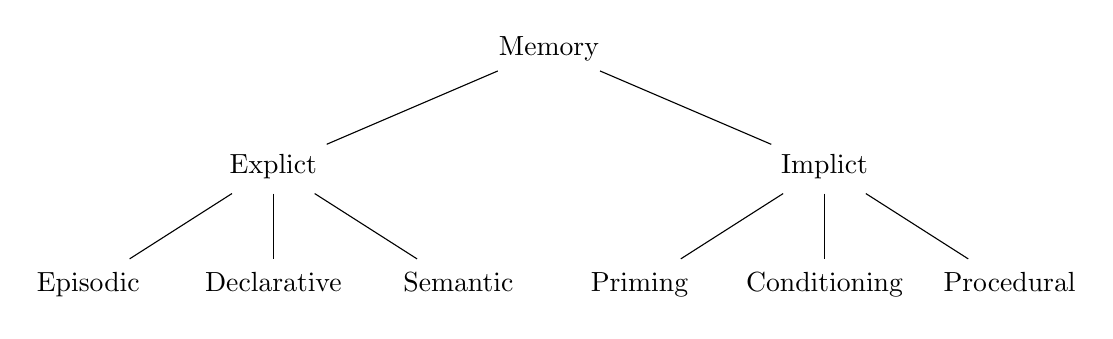
\begin{tikzpicture}
        [level 1/.style={sibling distance=7cm},
        level 2/.style={sibling distance=2.35cm}]
        \node {Memory}
        child {node {\strut Explict} child {node {\strut Episodic}} child {node 
                {\strut Declarative}} child {node {\strut Semantic}}}
        child {node {\strut Implict} child {node {\strut Priming}} child {node 
                {\strut Conditioning}} child {node {\strut Procedural}}};
    \end{tikzpicture}
    \caption{Categorization of memory by type of stored 
        information}\label{fig:memtypes}
\end{figure}


\section{Experimental findings in memory research}\label{sec:exp-findings}
Most memory experiments require the participants to memorize lists of words and recall them afterwards.
Usually an experiment will fall into one of two categories depending on how the subjects are required to recall the list items: in free recall experiments, the subjects are free to recall the items in any order; in serial recall experiments, the subjects are required to recall the items in order.

The hallmark finding in memory research, especially for serial recall experiments, are the \emph{primacy} and \emph{recency} effect.
Subjects tend to remember the start of list (primacy) and the end of list (recency) better (\cref{fig:exp-serial-pos}).
Furthermore, if subjects in a serial recall experiment recall an item at the wrong position, a so-called \emph{transposition}, it is more likely to be an item that was close in the list than an item several positions apart.
\begin{figure}
    \centering
    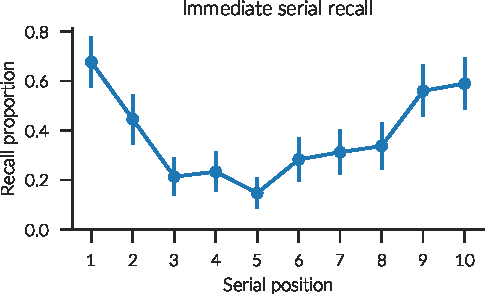
\includegraphics{figures/exp-serial-pos}
    \caption[Immediate serial recall position curve]{Serial position curve of a immediate serial recall experiment with a 10 item list. Data reproduced from \textcite{Jahnke1968} with \SI{95}{\percent} confidence intervals.}\label{fig:exp-serial-pos}
\end{figure}

In free recall experiments, a recency effect is observed as well.
This does not only show in the serial position curve, but participants often start out with recalling the last item first.
This can be measured by the \emph{probability of first recall} (\cref{fig:exp-free-recall}).
Another important aspect of free recall is captured by the conditional response probability (CRP).
It gives the probability for the difference (the \emph{lag}) in serial positions of two recalled items.
It is peaked around zero, indicating that items in proximity in the learned list tend to be recalled together, while jumps to remote items are rarer.
This is known as \emph{contiguity} or the \emph{lag-recency effect}.
The CRP curve also has a characteristic asymmetry which shows the bias for forward (opposed to backward) recall.
\begin{figure}
    \centering
    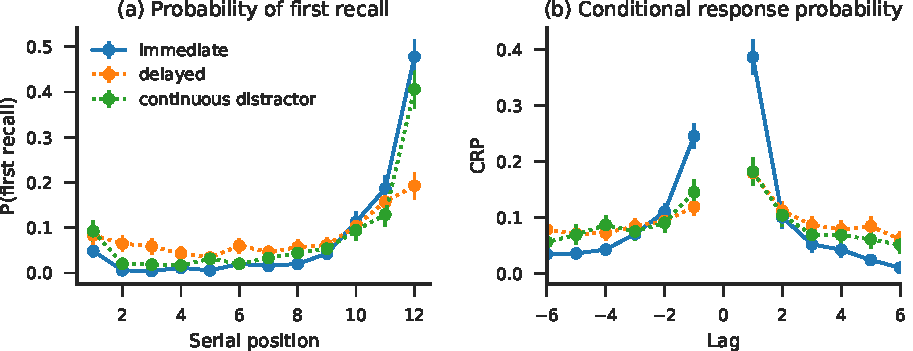
\includegraphics{figures/exp-free-recall}
    \caption[Free recall probablitiy of first recall and CRP]{Data from free recall experiments with 12 item lists. (a) Probability of first recall. (b) Conditional response probability. All data from \textcite{Howard1999} with \SI{95}{\percent} confidence intervals.}\label{fig:exp-free-recall}
\end{figure}

By introducing a delay filled with a distractor task, referred to as \emph{delayed (free) recall}, both the probability of first recall and the CRP curve will become much flatter.
This effect cannot solely be attributed to (suppressed) rehearsal effects as introducing an equally long distractor interval inbetween the list items, known as \emph{continuous distractor (free) recall}, partially restores the recency effect in the probability of first recall.

While there are many other experimental findings in memory research, there are two more findings that I will focus on in this thesis.
First, the differential effects of the acetylcholine antagonist scopolamine on encoding and recall \parencite{ghoneim1975}.
Recall performance is normal when scopolamine is injected after the presentation phase, but the number of successful recalls is considerably lower when the injection is done before the presentation phase.
The number of successfully recalled items in the later case is around the short-term memory span which might show an effect purely on LTM, but not STM\@.
This experiment is of interest as a neural network model is more suited to modeling such drug effects than typical mathematical models.

Second, the Hebb repetition effect the observation that in repeated immediate recall experiments, the recall accuracy of a repeated list (typically every third list) will increase with repetitions \parencite{Hebb1961}.
Whether the test subject has to become consciously aware of the repetition is debated \parencite{Stadler1993}.
It is of interest in this thesis the Hebb repetition effect has been regarded useful in testing interaction of STM and LTM, or as \textcite{Burgess2005} phrase it, it is  a ``powerful vehicle for developing and testing models of the relationship between STM and LTM''.


\section{Neuroanatomy of memory}
Short-term memory is attributed to cortical brain regions, but there is no single region that is the unique locus of STM\@.
Sensory short-term memory is distributed across the corresponding cortical sensory and related brain regions \parencite{zelano2009,todd2004,baldo2012}.
For example, auditory memory can be found in the temporal cortex close to speech processing areas, whereas visual short-term memory is located in parietal cortex.
Furthermore, multimodal integration and manipulation in working memory has been found to lead to increased activation in prefrontal cortex \parencite{rypma1999}.

Compared to short-term memory, the formation of new long-term memories is more localized.
In particular, the hippocampus (HC) has been implicated in the acquisition of new declarative and episodic memories \parencite{eichenbaum2001-1}.
A finding originally derived from patients with hippocampal lesions, most famously HM who got his hippocampus (but also other brain regions) removed due to severe epilepsy \parencite{penfield1958,scoville1957-1,squire2009}.
The hippocampus is named for its sea horse shaped structure.
It is located in the medial temporal lobe (\cref{fig:hc}) and neighbours the subiculum and entorhinal cortex (EC).
The hippocampus is further divided into substructures CA3, CA1, and the dentate gyrus (DG) by its cytoarchitectural structure.
While the CA3 and CA1 regions consist mainly out of pyramidal neurons and about \SI{10}{\percent} GABAergic, inhibitory interneurons \parencite{Freund1996}, granule cells are the main constituent of the dentate gyrus.
Furthermore, the dentate gyrus has a large number of cells compared to CA3 that exhibit sparse activity.
In humans the cell count of the DG is about twice as high as in CA3, whereas in rats DG has about five times more cells than the CA3 region.
\begin{figure}
    \begin{addmargin*}[0mm]{-70.16pt}
        \hfill
        \subcaptionbox{}{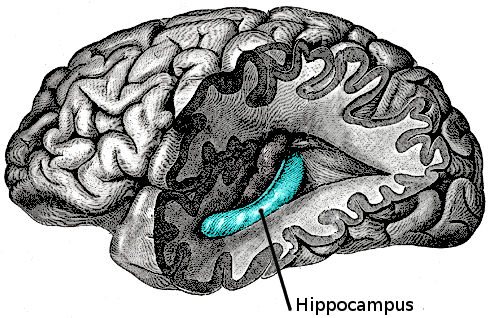
\includegraphics[width=2.45in]{figures/Gray739-emphasizing-hippocampus}}
        \hfill
        \subcaptionbox{}{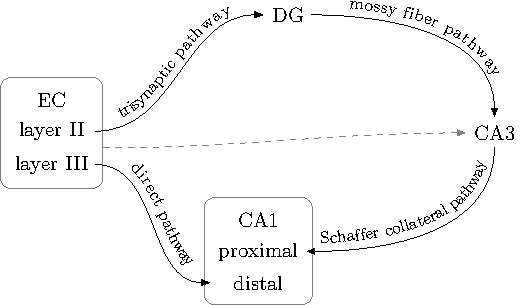
\includegraphics{tikz/hc}}
        \hfill
        \caption[Hippocampal anatomy]{(a) Location of the hippocampus in the human brain. (b) Connectivity between entorhinal cortex (EC) and hippocampal subregions: dentate gyrus (DG), CA1, CA3.}\label{fig:hc}
    \end{addmargin*}
\end{figure}

The connectivity to, from, and within hippocampus is exceptionally well known.
There are two major pathways from entorhinal cortex.
The \emph{direct pathway} originates in layer III of the entorhinal cortex and targets the distal apical dendrites of CA1 neurons.
The \emph{trisynaptic pathway} originates in layer II and leads via the dentate gyrus, and CA3 also to CA1, but targeting the proximal dendrites (a signal thus crosses three synapses).
The connections from the dentate gyrus to the CA3 region in this is termed the \emph{mossy fiber pathway}.
Each of these mossy fibers innervates about 15 neurons \parencite{Claiborne1986} which results in each CA3 pyramidal neuron receiving input from about 50 to 90 granule cells \parencite[230]{Squire1989}.
The final bundle of connections from CA3 to CA1 is known as the \emph{Schaffer collateral pathway}.
Further major hippocampal connections exist from the entorhinal cortex to CA3, mostly targeting the same cells as the connection from dentate gyrus \parencite{Paxinos2014}, and recurrent connections in CA3.
However, a single cell in CA3 is not recurrently innervated by more than 5\% of all CA3 cells \parencite[231]{Squire1989}.

Given these neuroanatomical properties, some of the hippocampal regions have been assumed to be involved in specific tasks.
The sparse coding and large cell count of the dentate gyrus led to the belief that it is responsible for pattern separation \parencite{Rolls2013}.
The CA3 region with its recurrent connectivity could be involved in pattern completion or forward predictions \parencite{Guzowski2004,Leutgeb2007,Rolls2013}.
Additional evidence for this comes from unimpaired recognition memory after lesioning the CA3 to CA1 connections despite impairing selective recall \parencite{Brun2002}. 

A review of hippocampal structures would not be complete without mentioning hippocampal place cells and entorhinal grid cells \parencite{hafting2005}, first discovered in rats, but existent also in other animals \parencite{buzsaki2013}.
A grid cell fires when the animal is a locations arranged in a regular hexagonal grid in an environment.
Place cells are similar, but fire only for one specific location in an environment and remap between environments.
While these cells are involved in navigational tasks, a connection to memory is possible \parencite{buzsaki2013}.
However, paying further attention to these cells is out of the scope of this thesis.

Closely related to grid and place cells is the hippocampal theta oscillation of \SIrange{4}{8}{\hertz} found in rats.
The spiking of place cells during a theta cycle is timed according to the distance from corresponding land marks, a phenomen termed \emph{phase precession} \parencite{okeefe1993}.
The coupling of the theta and gamma bands has also been shown to be important in the learning of item-context associations \parencite{tort2009}.
Despite some debate, there is evidence for similar, but slower ($<\SI{4}{\hertz}$), hippocampal oscillations in humans related to episodic memory encoding \parencite{lega2012}.
However, their functional relevance is not entirely clear at this point.

Finally, most commonly during sleep, but also in immobile rats, sharp waves (SPWs) are observed in the rat hippocampus \parencite{chrobak1994,girardeau2009}.
These have been implicated to be involved in memory consolidation from hippocampus to the neocortex, a process not covered in this thesis.


\section{Memory models}
Different memory models can be roughly sorted into three classes.
Conceptual models describe different components and processes of memory and their interaction.
Often they will be presented as box and arrow diagrams.
They do not allow for a precise mechanistic explanation or quantitative predictions.
Mathematical models address this by providing exact equations that can be evaluated to obtain quantitative predictions.
However, they do not explain the neural implementation and thus are not constrained to biological plausible mechanisms.
Finally, connectionist models use neural networks with varying degree of abstraction.
As such their biological plausibility also varies.
While those models come closer to explaining neural mechanisms of memory, they less often address the behavioural data from high-level cognitive experiments.

\subsection{Conceptual models}
\Textcite{Yntema1963} presented one of the first models of memory.
They conceptualized retrieval as a search process where each item in memory is associated with tags referencing further information.
For example, a time tag would encode the time an item was observed.
The whole description, however, is more based on how a memory system could be implemented on a classical von Neumann computer and does not consider if or how those operations could be neurally implemented.

To date, the most influential conceptual organization of working memory was proposed by \textcite{Baddeley1986}.
He proposed, based on experimental data, separate stores for visual and acoustic information, termed the \emph{visuospatial sketchpad} and \emph{phonological loop} respectively.
These are controlled by a \emph{central executive}.
Furthermore, in \textcite{Baddeley2000} the model was extended with an episodic buffer for the binding of multimodal information and transfer to episodic long-term memory.
The main relevance of the model is that it informs us about the organization of (working) memory by modality; but it does less to elucidate mechanisms.

In general, conceptual models can give a high-level account and they can be evaluated with respect to their qualitative agreement to behavioural data.
However, they cannot provide us with quantitative predictions which makes a more rigorous validation difficult.
They, also, do not explain the cognitive mechanisms in detail and an account of the neural implementation is completely out of their reach.


\subsection{Mathematical models}
Some of the weaknesses of conceptual models are addressed by mathematical models.
These models will make quantitative predictions about the behavioural data and describe underlying cognitive mechanisms to a varying degree, but do not provide a neural implementation.
There is a vast amount of such models and not all can be discussed here.
Thus I will focus on the most influential ones.

That list certainly contains the perturbation model for serial order by \textcite{Estes1972}, the free recall model Search of Associative Memory (SAM) by \textcite{Raaijmakers1981}, the recognition memory model Retrieving Effectively from Memory (REM) by \textcite{Shiffrin1997}, and the episodic memory model MINERVA2 by \textcite{Hintzman1988}.
The perturbation model is an early attempt to provide a mathematical framework of how remembered item positions can drift over time.
In SAM cues are assembled in a short-term memory to retrieve associations from a long-term associative memory (the search part of the model).
In the REM model error prone copies of feature vectors derived from the study items are stored.
A recognition probe is matched to the stored feature vectors and a likelihood ratio of the match scores being generated by an old versus a new item is calculated.
The MINERVA2 model also uses feature vectors that are stored as traces and can be probed by cues.

All of these models, and most other mathematical models, either assume item-to-item or position-to-item associations.
The primacy model by \textcite{Page1998} is worth noting because it uses a different approach.
In that model items are activated according to a primacy gradient, but the model is agnostic to how this gradient is generated.
This, however, also leaves that aspect underspecified.

Common to all of these models is that they are not demonstrating biological plausibility.
Thus it is unclear, whether any of the models can be implemented in a neural substrate while preserving the predictions.
Or even if, what the limitations with regard to noise and requirements for neural resources are.
Nevertheless, mathematical modelling is an important first step in figuring out what sort of processes are worth considering for a neural implementation.
Also, there are some reoccurring ideas in these models that are useful to consider in the context of a neural model.
For example, starting with \textcite{Anderson1973} many models have used random feature vectors to represent individual items.
That approach is similar to the Semantic Pointer Architecture (SPA) presented in \cref{sec:spa} which can be implemented neurally with the methods of the Neural Engineering Framework (\cref{sec:nef}).

An especially influential model based and random feature vectors was \mbox{TODAM2} \parencite{Murdock1993}.
It was able to fit a large body of experimental data and in that aims to be a general theory for item recognition, serial order, and associative memory.
A neural implementation could very well be possible with the NEF, but has not been attempted so far.
However, \textcite{Choo2010} pointed out that the dimensionality of the vectors in the model increases with each stored item.
Thus, the requirement for neural resources grows unbounded.
It also worth noting, that \mbox{TODAM2} does not give an account of how responses are generated.

Another useful idea, that had its origin in mathematical models, is the idea of a randomly drifting context signal that items get associated to.
\Textcite{Estes1955} presented the first model of this type and \textcite{Murdock1997} extended the \mbox{TODAM2} model in this way to explain additional data.
An open question in these sort of models is, how the context at an earlier time can be re-instantiated to start the recall and how the context is advanced in the same way during recall as in the study phase to recall the remaining items.
As the signal drifts randomly a memory for the context signal itself would be needed.
The OSCAR model \parencite{Brown2000} solves part of this by using a deterministic context signal that is generated from multidimensional oscillators.
This allows to replay the exact same context signal once it has been reset.
It still does not answer how the context is re-instantiated to start the recall as this still requires knowledge of the oscillator states at begin of the study phase.

All of these context-based models cannot explain the asymmetric CRP curves.
The temporal context model \parencite{Howard2002}, however, was specifically constructed to explain these free recall data.
It also uses a context signal, but this signal is updated by the studied (and recalled) items themself.
Each item recalls a prior context associated with that item to partially update the current context and the updated context gets associated with the studied item.
This solves the re-instantiation problem as the right cue can set the context to be similar to the study context to retrieve an item.
That retrieved item in turn updates the context to retrieve more items related to the updated context.
Thus, it is also available to appropriately advance the context after each recall.
The model will discussed in more detail in \cref{sec:tcm}.
But the TCM is not perfect.
It did not capture immediate free recall data involving short-term memory, even though it was presented as a single-store framework, i.e.\ a single memory for both STM and LTM\@.
This single-store assumption was criticized by \textcite{Davelaar2008} and is in contradiction to neuroimaging data \parencite{talmi2005}.

Many of these models are also vague on the exact processes of recall.
Though, the ACT-R model of serial recall by \textcite{Anderson1997}, in which items are associated with their serial positions, describes detailed steps necessary for recall.
Unfortunately, it is vague on the exact storage mechanism of items.

Recently, \textcite{shankar2013} proposed an \emph{optimally fuzzy temporal memory} that is less motivated by behavioural data, but more by a mathematical optimal and scale-free storage of a time-varying signal.
Nevertheless, it has been proposed to model the coding in hippocampus \parencite{howard2014-1}.
In this framework, the input signal is stored by a bank of leaky accumulators with different time constants.
This corresponds to a Laplace transform of the signal.
To decode the history of the input signal, a linear operator approximating the inverse Laplace transform is used.
I will discuss this model in more detail in Section TODO, and demonstrate that it is highly sensitive to noise which is prohibitive to a neural implementation.


\subsection{Connectionist models}
Compared to the vast amount of mathematical models, there are much fewer connectionist models that try to ensure more biological realism.
Many of these models focus on reproducing low-level findings in the hippocampus such as sequence compression in replay \parencite{Levy2005} or place cells \parencite{Milford2004}.
The model presented by \textcite{Hasselmo2012}, might very well be the most comprehensive hippocampus model to date, describing the storage of episodic memories as a spatial trajectory.
It addresses experimental data on place cells and the theta rhythm.
A very recent model by \textcite{yu2017}, constructs a three-layer spiking neural network that is able to encode a sequence over several iterations and replay it during a cycle of the theta rhythm.
These models, however, still leave a large gap to high-level cognitive behaviour as modelled by mathematical models.
In addition, the \textcite{Hasselmo2012} relies on hypothetical ``arc length'' cells to disambiguate memories \parencite[cp.][]{Robins2014}.

Nevertheless, there are some connectionist models that try to reduce this gap by addressing behavioural effects with a neural network implementation.
Namely, \textcite{Burgess1992} and \textcite{Burgess1996} proposed models for the articulary loop, \textcite{Norman2003} for recognition and familiarity effects, and \textcite{Botvinick2006} for immediate serial recall.
All of these models use rate based neurons as an abstraction.
While rate neuron models are a useful tool to build tractable models with a degree of biological realism, one has to be careful to not introduce biologically implausible features.
For example, the noise introduced by discrete spikes is neglected.
In particular, \textcite{Norman2003} use a $k$-winner-take-all mechanism that is hard to realize in spiking neurons as it requires a fine balance of excitation and inhibition.
Potentially even more problematic is the use of back-propagation learning in the model by \textcite{Botvinick2006}.
While learning with back-propagation is a tremendously successful technique in machine learning, it is still unclear whether biological neural networks can implement this sort of learning.
But new techniques like feedback-alignment \parencite{lillicrap2016} and related work \parencite{bengio2015} might provide biological plausible implementations.

I only know of two memory-related models that address these concerns about biological plausibility by using spiking neurons while at the same time connecting to behavioural data.
The first one is the ordinal serial encoding (OSE) model of serial recall by \textcite{Choo2010}.
As a primarily short-term memory model, it uses recurrently connected neurons to store the memory trace in neural activity.
This approach is also used to model a long-term memory component that can be attributed to hippocampal storage.
While this allows for a first approximation, a storage in synaptic weights seems more realistic for such a component.
The second model was specifically developed to model the storage of serial lists with hippocampus by \textcite{OliverTrujillo2014}.
It is able to reproduce neural data like replay and theta rhythm.
However, the length of stored lists is limited in similar fashion to the STM capacity in the OSE model, despite long term memory being certainly able to learn longer lists.
Learning longer lists in the model would require the chaining of individual lists with different contexts, but no mechanism for this has been given in the model.
Another questionable feature is the usage of a clock signal that is adjusted to speed up compressed replay.


\subsection{Summary}
Despite many existing models, a number of questions has not been sufficiently addressed \parencite[cp.][]{horwitz2008}.
To date no model demonstrates a satisfying degree of biological plausibility while at the same time addressing behavioural data from cognitive psychology.
Many models are not concerned with the interaction of short-term and long-term memory despite the importance for many fundamental effects on memory performance.
This includes neural processes for the coordination and control of the interplay of these memory components.
Finally, the recall process or reinstantiation of recall context is often not precisely explained even though it is an essential part of memory function.

I address these points with the context-unified encoding (CUE) model presented in this thesis.
It combines activity-based short-term memory with weight-based long-term memory and also specifies the required control and recall processes.
Biological plausibility is ensured by an implementation as a spiking neural network.
Despite the low-level implementation, it is validated against human, behavioural data.

This thesis is divided into two parts.
In the first part, all the basic methods required for the construction of such a large-scale spiking neural network model are given.
This includes some secondary research objectives to improve neural representations to ultimately require less neurons for a higher simulation throughput.
In the second part, the methods from the first part are employed to build up the actual CUE model and compare the model predictions against human data.
